\newpage
\chapter{Изработване на електронна игра}
\label{chapter02}

За разлика от много операционни системи Symbian първоначално е създаден за персонални компютри, а не за мобилни устройства. Това води до някои от предимствата на Symbian OS - той е оптимизиран на ядрено ниво с ниска производителност, за да работи с критично важни устройства, заемайки минимална памет. Symbian OS е потомък на операционната система EPOC 16-битова еднопотребителска многозадачна операционна система, която е разработена от Psion за тяхните лаптопи SIBO (Sixteen Bit Organizer) през 1989 година. Названието EPOC е съкратено от „Епоха“ или по точно от Electronic Piece Of Cheese. Написана е на асемблер (Intel 8086) и C, поддържа разработката на C и OPL приложения, използвайки IDE OVAL (Object-Based Visual Application Language), както и графичен интерфейс (по този начин пред Microsoft Windows 3.0). Впоследствие, EPOC OS е напълно преработена за първи път от PDion Series 5 PDA, като наименованието не се променя особено - EPOC / 32 OS. Впоследствие Psion Software се ангажирана с подръжката и непрекъснато подобряване. Софтуерът на Psion, Nokia и Ericsson създават Symbian Ltd през 1998 г. Целта на новият софтуерен продукт е да разработва нова операционна система от световна класа за модифицирани устройства, базирани на PDA и телефони. Акционерите на Symbian Ltd, Panasonic, подобряват версията с виртуална машина Java ME, обновяват функцията/работата по подразбиране с Unicode низове.

Няколко години по-късно Sanyo и Sony се сдобиват с лиценза върху Symbian, като обявяват на пазара първата официална версия- Symbian смартфон, който съчетаваше организатор и мобилен телефон в едно. Symbian се развиха доста добре на пазар, но през 2004 г. става ясно, че PDA  система вече я няма. Psion продава своя дял в Symbian Ltd и накрая закрива производството. 

Symbian Ltd продължава да се бори в технологичното производството и за пазара. Не след дълго придобиват лиценз за ползването на Microsoft Exchange Server Active Sync протокол. Пускането на новата версия Symbian OS 9.1 е със защитен модул, който изисква задължително автентикация и сертификати преди инсталиране на приложение. По същото време се появяват  конкурентни устройства с нова операционна система, който са поддържани от платформата UIQ3. Въпреки това компанията не отстъпва, като започва усърдно разработване на нови процесори, платформи, ъдейти, университетски платформи, многоядрени процесори за цифрова телевизия в DVB-H и ISDB-T формати. Голяма подкрепа указват Nokia, Sony Ericsson, NTT DoCoMo и Samsung с дарението на ресурсите и изходните кодове на платформите S60, UIQ и MOAP., с резултат от над 200-милионна продажба на мобилните устройства с операционна система Symbian. В началото на 2009 г. компанията обявява прекратяване върху поддръжката на платформата UIQ и публикуван изходният код от микроядрото на EKA2 Symbian OS. През цялата история на Symbian OS са пуснати в продажба повече от 250 модела и устройства под негов контрол от дузина производители с общо над 250 милиона.

Двамата студенти по инженерни науки Майк Лазардис и Дъглас Фреган регистрират собствена фирма Research In Motion (RIM) в Канада. Първоначалната дейност е свързана с пренос на данни, а първият продукт представлява двупосочен пейджър за имейли. Устройството е иновативно за времето си, но истинският успех на компанията идва с първите й смартфони, които имат големи и удобни QWERTY клавиатури. Именно дизайнът и удобната клавиатура, наподобяващи  семки на къпина дали името BlackBerry.

През първата половина на новото десетилетие RIM е истински лидер при смартфоните в САЩ и Канада устроено за имейл, главно ориентирано за бизнесмени. За младите хора и като цяло за всички, които не работят в корпоративния сектор е безинтересен. Основното предимство на BlackBerry е BBM, все още е една от най-стабилните IM платформи, а BlackBerry Email е избор на редица бизнес корпорации заради високото си ниво на сигурност. Това изстрелва RIM в класацията на най-бързо развиващата се компания в света, като приходите се увеличават с 84\% за три години. 50 милиона смартфона са продадени за десет години, което прави BlackBerry вторият най-популярен смартфон в света. Вдъхновена от успеха, RIM решават да излязат извън корпоративния пазар и започва да създава „умни“ приспособления, които обикновените канадци и американци биха могли да ползват.

Доминираща компания в сектора за безжична електронна поща, RIM губи пазарен дял поради ожесточената конкуренция от страна на Apple Inc. iPhone и телефони, работещи с Google Inc . Android софтуер. Спадът е повлиян с обявяването на стратегическото преструктуриране в пазарния сектор. Макар и твърде късно, ръководството на BlackBerry осъзнава, че битка е загубена и компанията трябва да се конкурира с новите играчи, идващи от IT сегмента, а правилата се налагат от Apple и Google. RIM успя да запази марката и да увеличи аудиторията си благодарение на добре разработените уеб услуги за подобряване на бизнес дейностите. С Интернет услугата BlackBerry (BIS), предназначена за малки предприятия, е отговаряла за синхронизирането и компресирането на данни в реално време, за да ускори изтеглянето и спестяването на Интернет трафик, както и защита на поверителността.
Първата повратна стъпка на пазара е с обявяването на Tablet PC, които технически характеристики оказват прогресивен успех: гумирано тяло, IPS-екран, ARM Cortex-A9 двуядрен процесор и високи басови високоговорители на предния панел.

Въпреки разработването на доста интересни смартфони, новото ръководство на RIM не успя да пребори конкурентния пазар. През септември на 2013 година RIM обявява, че напуска потребителския сегмент на пазара за мобилни устройства. Сега BlackBerry отново е разработван зад параван с това, което първоначално започна: да проектира хардуерни и софтуерни приложения и услуги насочени към корпоративния сектор.

Постоянната еволюция при мобилните устройства, високата конкуренция за иновативност и голям пазарен дял повлиява върху развитието на смартфоните. Съчетаването на услугите между персонален компютър и смартфон представя новият модел Pocket PC, като съхранява голяма  информация  достъпна по всяко време и от всяко място. Устройството замества смартфоните, таблетите, лаптопите чрез софтуера си даващ достъп до много операции за ползване като: калкулиране, часовник и календар за планиране на времето и задачите, адресна книга, игри, достъп до Интернет, получаване и изпращане на електронна поща,  текстообработка, видеозаписи, слушане на радио, GPS, слот за карта с памет за съхраняване на данните и IrDA(инфрачервен порт за свързване чрез  Bluetooth и Wi-Fi) порт за връзка служещ за високоскоростен обмен на данни, включват нови потребителски интерфейси и т.н.

Въведена нова версия от Windows Mobile- Pocket PC програмистите внедряват основен комплект на софтуер за работа в офиса, приложения за развлечения като Windows Media Player 8 и безжични модули(L2TP / IPsec VPN,Phone Edition и други). От техническа гледна точка Pocket PC е спецификация на Microsoft, която специфицира различни хардуерни и софтуерни изисквания за мобилни устройства. Оригиналната операционна система Pocket PC e сходна с Windows 98, Windows Me и Windows 2000 операционни системи и със специфични няколко процесорни архитектури: SH-3 , MIPS и ARM. Windows устройството съдържа множество вградени приложения като Microsoft Reader , Microsoft Money, Pocket Internet Explorer, Windows Media Player, Pocket Word, Pocket Excel и Pocket Outlook за да се подобри нивото сред конкуренцията.

Въпреки силният маркетинг, вградените функционалности и приложения пазарният дял търпи спад. Агресивният маркетинг от страна на Apple и Android Google срива новодошлите компании сред мобилните устройства. През октомври 2017 г. корпоративният вицепрезидент на Microsoft Джо Белфиоре потвърди, че вече няма да продават или произвеждат нови мобилни устройства. Съществуващите устройства ще бъдат поддържани и следени за възникващи грешки, които ще бъдат поправяни,а  защитата актуализирана.

С еволюцията на човечеството, светът се развива на бързи обороти. Промените и новостите навлизат в бита и ежедневието. Съвременният свят е немислим без технологиите, а най-разпространената и употребявана е гъвкавата комуникационната връзка между хората, не зависимо на коя точка от света са, която предоставят мобилните устройства.

Идеята за мобилната връзка е възникнала през 1920г., която главната цел за мобилната връзка е била да подобрява обществените услуги като бърза помощ и различни диспечерски услуги, а по-късно навлиза и в бизнеса. През периода на 50-те и 80-те се развиват полупроводниковите системи и започва началото на автоматизирането на мобилната връзка чрез радио системата. Но истинското развитие на мобилните комуникации води началото си с разработването и прилагането на клетъчните системи още през 70-те, като първия мобилен телефон е на лице и готов за употреба през 1973г.

Всъщност първият мобилен телефон е вдъхновен от филм, който показва технологията на мобилната връзка като нещо от далечното бъдеще. Малко по-късно, когато филмът Стар Трек вдъхновява Мартин Купър през 69г. той започва първите си опити за разработването на мобилен апарат и 14 години по-късно през 83-та на пазара е първият мобилен телефон Dynatac 8000X0 на Моторола. Телефонът е с доста голям размери, също така е тежък, което го прави неудобен и същевременно е скъп. Теглото му е около килограм, а цената около 4 хиляди долара. Това голямо чудо на техниката е било доста неудобно за носене и далеч от реалната концепция. Макар и технологията да е революционна размерите на апарата са голям минус за успешното му разпространение на пазара.

В България мобилните технологии навлизат началото на 90-те под формата на мобифони, които са поне на половина по-леки от първият мобилен телефон. Основния клиент на устройствата и услугите са бизнес служителите, устройството все още не е стигнало до масовия, обикновен потребител. Няколко години по-късно технологиите започват да се развиват с доста по-голяма скорост и обема на мобилния телефон достига размерите на слушалка от обикновен стационарен безжичен телефон.

За краткия период на своето развитие безжичните клетъчни комуникации претърпяват съществени изменения и не само количествени, но и качествени, които продължават и до днес. Това дава основание да се говори за три поколения мобилни клетъчни системи: първо поколение – аналоговите системи, постепенно отмиращи в миналото;
второ поколение – цифровите системи на днешния ден; трето поколение – универсалните системи за безжични връзки на недалечното бъдеще.

Във всички аналогови мобилни клетъчни системи се използва честотна модулация за предаване на речта и служебната информация (или сигнализацията). Предаването става по радио канали, които използват различни участъци от честотния спектър. Основният недостатък е относително малкият капацитет (това е следствие на недостатъчно рационалното използване на заделените честотни ленти при честотното разделяне между каналите). Този недостатък е е бил забелязан в средата на 80-те години, първоначално в страните с най-широко разпространени мобилни клетъчни връзки. Дефектът предизвиква търсенето на по-съвършени технически решения. В резултат на тези усилия са се появили цифровите мобилни клетъчни системи от второ поколение. Преходът към цифровите системи се е стимулирал и от широкото внедряване на цифровата техника в телекомуникациите. В значителна степен преходът е подпомогнат от разработването на ниско скоростни методи за кодиране и появата на свръх миниатюрни интегрални схеми за цифрова обработка на сигнали. Всички цифрови системи от второ поколение се характеризират с по-ефективно използване на наличния честотен спектър, съществено разширение на възможностите за управление и поява на допълнителни функционални възможности.

Системите от трето поколение предлага безжична връзка за всички видове телекомуникационни услуги. Те се интегрират с информационните услуги и предлагат широк набор от възможности за мултимедия, видео конференция, високоскоростен достъп до Интернет, предаване на делова, развлекателна и образователна информация и т.н. С достъп до всяка услуга навсякъде и по всяко време разрушава съществуващата ограничаваща граници за комуникация, информация, достъп до медиите и други забавления. Мобилната телефония дава възможност за разговор, докато човек извършва най различни движения. Световната мрежа Интернет превърна прехвърлянето на данни в полезни и лесни за използване услуги. 

Последните няколко години операционната система Android, си извоюва мястото на най-популярна мобилна операционна система в света и също така стана в лидер при таблетите.

Android Inc. е основана 2003 г. от Анди Рубин, Рич Майнър, Ник Сиърс и Крис Уайт. Първоначалната идея на компанията е да създадат операционна система за цифрови фотоапарати, която да позволи на устройствата да се възползват от функции като гео-тагване. Създателите бързо проумяват, че пазарният дял на фотоапаратите е прекалено малък и пренасочват продукта си към операционна система за смартфони, която да бъде конкурентна на тогавашните лидери на пазара – Symbian и Windows Mobile. Въпреки добрата идея и екипът специалисти, компанията има финансови затруднения и две години след създаването си Android Inc. е пред фалит. През 2005-та Google проявява интерес към младата компания и пръв инвестира, а в последствие придобива Android. Рубин, Майнър и Уайт остават в управлението на компанията и стават служители на Google.

Първото официално устройство, налично в търговската мрежа, което използва операционната система Android, е HTC Dream. Макар и много от функциите да липсват (като виртуална клавиатура и multi-touch), HTC Dream и Android 1.0 показват за първи път някои от най-популярните и ключови парадигми и елементи на дизайна, които се превръщат в запазена марка на операционната система и Google. Първото обновяване на системата, пък, се случва през април 2009 година: тогава и започва традицията всяка следваща версия на Android да носи име на сладкиш ( например първият ъпдейт е наречен Cupcake („кексче”), а следващи ъпдейти с имена като Eclair (еклер), Froyo (десерт с йогурт) и други ).

Операционната система вече се е доказала като гъвкава и адаптивна, а освен таблети и смартфони, Android днес управлява най-различни потребителски устройства – от телевизори и гейм конзоли до фитнес тракери и автомобили. 

Най-модерната операционна система в света, разработена от Стив Джобс, преобръща представата в технологичната индустрия. iOS е мобилна операционна система произвеждан от компютърния гигант Apple Inc. За първи път е вградена в мобилното устройство Iphone и представен от главния изпълнителен директор (Стив Джобс). Още в първата версия на операционната система (iPhone OS) са създадени много съществени функции  на софтуера. Отличителната иновативна технология, която го отличава и популяризира спрямо останалите устройства, извеждайки го в класацията като най-търсената мобилна операционна система в света до ден днешен е оригиналният хардуер, който не позволява работа на iOS с други и различни хардуери. С първата версия Apple налага Spring Board – решетката от приложения на екрана и мулти тъч, като основна идея на компанията е да могат да функционират успешно и едновременно с iPod, камерата, мобилните разговори и Интернет конзолата, съчетавайки всичко изброено в малко устройство, побиращо се в джоб. Apple разработват интерфейсът на iOS, който на места наподобява физически обекти ( например, бележките са много идентични с истинска тетрадка ). Той е базиран на концепцията за директна манипулация- мулти-тъч движения , който се състоят от плъзгащи, ключови и бутони визуализации. С помощта на флуиден интерфейс (гладък/изчистен интерфеис) се управляващи устройството, като екрана реагира веднага на всяко  движение от пръстите. 

Със създаването на нови версии и модели iPhone се появяват нови приложения, като iCloud. Първият за онова време облак, които функции са да събере и прехвърли всички данни от смартфона,  чрез iTunes. Следващата голяма крачка, която Apple правят за да утвърдят на пазара е с въвеждането на App Store. Програмистите разполагат с индивидуални за Apple инструменти чрез които разработват програми и приложения, които работят само на Iphone. Това е главна причина интересът да се поддържа толкова дълго време на това високо ниво. Операционната система iOS се припокрива с основната операционна система на компютрите Mac - Mac OS X, но двете нямат съвместимост помежду си.

Поредният иновационнен бум сред мобилните устройства, който прави гиганта е с гласния асистент и навигатор Siri. Приложението комуникира с всички останали приложения, но и с други допълнителни устройства. Нововъведението изпълнява гласовите  команди на потребителя, като например повикване или да изпрати съобщение на някого, да отвори приложение, да търсене в Интернет, за справка на  информация, за търсена на локации,  да отговори на общи въпроси и други най-различни задачи.
Също така спечелиха нови. Компанията пробива музикалният пазара за стриминги и предоставя на музикалните артистите със собствено оборудване използват корпоративни услуги: Apple Pay и Apple Music.

Apple развиват технологичното си многообразие спрямо тенденциите в информационните технологии разработвайки своя собствена система за интелигентен контрол на домовете, като  и програмата Health, която дава точни данни за физическото състояние на потребителя. Всяка година се пуска по една основна версия, а и с тях иновациите в технологиите.

\section{Избор на развойни средства}

Програмният език Objective-C е създаден от Брад Кокс в началото на 80-те години, който е обектно-ориентиран език за програмиране основан на предаване на съобщения към обектни инстанции и е разширение на езика C. Той добавя Smalltalk- стил съобщения, който може да не се изпълняват, а когато методът разрешен за изпълнението от кода. Например, съобщение се изпраща към колекцията от обекти, на които само някои отговорят, без да се създават на грешки по време на изпълнението. Предаването на съобщения също не изисква да се дефинира обект по време на компилация. Objective-C се разширява в NeXT с цел да бъде въведена концепцията за множествено наследяване от спецификации чрез въвеждането на протоколи, но без да се реализират. Този е модел може да се постигне или като абстрактно множество от наследен базов клас в C ++  или като интерфейс (както в Java и C\#).

NeXT Software лицензира езика и разработва библиотеки с кодове, наречена NeXTSTEP(който след това поддържан Apple). Когато Apple Computer се сдобиват с NeXT, библиотеката от кодове на NeXTSTEP е вградена с ядрото от операционната система на Apple, Mac OS X. NeXTSTEP предоставя на Apple модерна OS основа, която Apple не може да разработи самостоятелно. Операционната система на iPhone, която в момента се нарича iOS, се базира на намалена версия на OS X. Следователно iOS наследява голямата част от библиотеката с кодове NeXTSTEP, както и обширна модификация и оптимизация. Тъй като NeXTSTEP е написан от Objective-C, iOS улеснява разработчиците на OS X да създават приложения за iPhone и iPod Touch. Това дава на програмистите гъвкавостта да се адаптират към бъдещите проекти съпоставени с минали, което ще доведе но висока функционалност и търсена на предстоящите продукти. Тази комбинация от функции - категории, протоколи и динамично изпълнение - позволява с помощта на NeXT да създаде AppKit, обектно-ориентирана библиотека за разработване на графични приложения, която все още Apple работи и до днес. Софтуерите  написан в Objective-C, спомагат на почти всички основни нови продукти: Mac OS X, iPhone, iPad, AppleTV и Apple Watch.

Историята на Objective-C и NeXT показва силното влияние на потребителите върху развитието на технологиите. До 1995 г. Objective-C е бил собственост и произведен от Stepstone, а NeXT  негов потребител. Независимо от това, NeXT успя да промени Objective-C за да задоволи нуждите и интересите на Apple, като в крайна сметка трансформира езика за iPhone на който се разбработва и до днес.

Swift е много парадигмен език за програмиране с модерна методология, предназначена за заместване на C-базирани езици (C, C ++ и Objective-C), предназначени за iOS, OSX и WatchOS, както и за работещи frameworks на Apple. Той е лесно достъпен и усвоим език за писане на софтуер, независимо дали е за телефони, настолни компютри, сървъри или каквото и да е друго устройство. Това го прави безопасен, бърз и интерактивен език за програмиране, който съчетава най-доброто в съвременното синтактично кодиране с по-широката инженерна алгоритмична архитектура и с голям принос за Apple и за разнообразната общността програмиращи с отворен код. Swift е предназначен да бъде по-устойчив на бъгове, благодарение на Objective-C, но като обем е по-сбит. Изграден с LLVM компилатора, включен в Xcode 6 и по-късно и използва средата на изпълнение Objective-C, която позволява на C, Objective-C, C++ ,му позволява компилацията на кодът да се изпълнява на една програма.
Развитието на езика Swift започнато през 2010 г. от Chris Lattner програмист в Apple. След дълга обработка едва след четири години по-късно приложението Worldwide Developers Conference (WWDC) стана първото публично публикувано приложение, написано на Swift. Бета версия на езика за програмиране е пусната на разработчици от Apple, но компанията не обещава, че окончателната версия ще бъде съвместима с на тестовата версия. Но очакванията са оправдани. Swift Programming Language е безплатно ръководство от 500 страници, което е пуснато в WWDC, също така достъпно на iBooks Store и на официалния сайт Apple Incorporation. Swift печели първо място за най-желан и предпочитан език за програмиране, а  Google обмисля да го използва като основен програмен език за Android. С традицията на Apple да заключва езиците към собствената си еко система, намеренията на Google може би няма да се осъществят. Apple иска да бъде на първо място на пазара, а отвореният код, който и дава ключово предимство за момента е Swift, а това го прави част от тази стратегия.

Първоначално Java е била проектирана за интерактивна телевизия, но е била твърде напреднала технология за индустрията на цифровата кабелна телевизия по това време. Историята на Java започва с Green Team. Членовете на екипа Джеймс Гослинг заедно с двама други Mike Sheridan и Patrick Naughton, докато те работят в Sun Microsystems (известни още като Green Team), инициират проект за разработване на език за цифрови устройства като телевизионни декодери, телевизори и т.н. По-късно от Netscape е включена Java технологията. Принципите за създаване на Java програмиране са: опростено, стабилно, преносимо, независимо от платформата, защитено, високопроизводително, многонишково, архитектурно неутрално, обектно ориентирано, интерпретирано и динамично. В момента Java се използва в Интернет програмирането, мобилните устройства, игрите, решенията за електронния бизнес и куп други приложения.

Java възможностите са не ограничени до конкретен домейн на приложението, а може да се използва в различни области на приложение и следователно се нарича Програмиращ език с общо предназначение. Кодът на Java не зависи от архитектурата на процесора. Приложенията на Java се компилират на 64-битова архитектура на всяка платформа, но също така и на 32-битова (или друга архитектура) система без никакъв проблем. Съществуват главно 4 вида приложения, които могат да бъдат създадени с помощта на Java. 

Самостоятелните приложения са известни и като десктоп приложения. Това е традиционен софтуер, който трябва да инсталираме на всяка машина. Примери за самостоятелно приложение са Media player, antivirus и др. AWT и Swing се използват в Java за създаване на компютърни приложения. 

Приложение, което работи на сървъра и създава динамична страница, се нарича уеб приложение. В момента технологиите Servlet , JSP , Struts , Spring , Hibernate , JSF се използват за изграждането на уеб приложения в Java.

Приложения, които са предназначени за предприятията и корпоративния бизнес , като банкови приложения. Java е с предимство за високо ниво на сигурност, балансиране на натоварването и клъстеризация. 

Приложения създадени за мобилни устройства. В момента се възползва Android от Java ME. Популярността на Java се появява с J2ME (сега известен като Java Micro Edition), която платформа  осигурява стабилна, гъвкава среда за приложения, работещи на вградени и мобилни устройства в Интернет, както и на: микроконтролери, сензори, портали, персонални цифрови помощници (PDA), телевизори топ кутии, принтери и др. Много функционалните и гъвкави потребителски интерфейси осигуряват стабилна сигурност, вградени мрежови протоколи и поддръжка за  офлайн приложения, които могат да се изтеглят динамично. Java се вписва в редица места на съвременния свят. Изпълнява се като самостоятелно приложение, уеб приложение, корпоративно приложение и мобилно приложение. Игри, смарт карти, вградена система, роботика, настолен компютър и др. Java е навсякъде.

Kotlin е статично типизиран език за програмиране, който се изпълнява на Java виртуалната машина и може да бъде компилиран в JavaScript кода или да използва LLVM инфраструктурата на компилатора. Основното му развитие е от екип от програмисти на Jetbrains, базирани и разработен за една година в Санкт Петербург, Русия. Основната цел за създаването му е за да стимулира продажбите на IntellieJ IDEA. Google обявява лиценз върху Kotlin с първокласна поддръжка за Android.

Като технологични характеристики биват разширени. Синтактично размерът на код е намален. Използвайте съществуващите библиотеки за JVM, Android и браузъра

\subsection{Избор на развойни инструменти}

\section{Стратегии за проектиране}

\subsection{Трислоен софтуерен модел}

Съвременните тенденции за разработка на софтуер често залагат на многослойни архитектурни решения. Един от най-популярните модели е с три слоя (Фиг. \ref{figure03}). Деленето на трите слоя обхващат визуализацията, обектно-ориентираният модел на данните и съхранението в енергонезависима памет (релационен модел). 

\begin{figure}[h!]
 \centering
 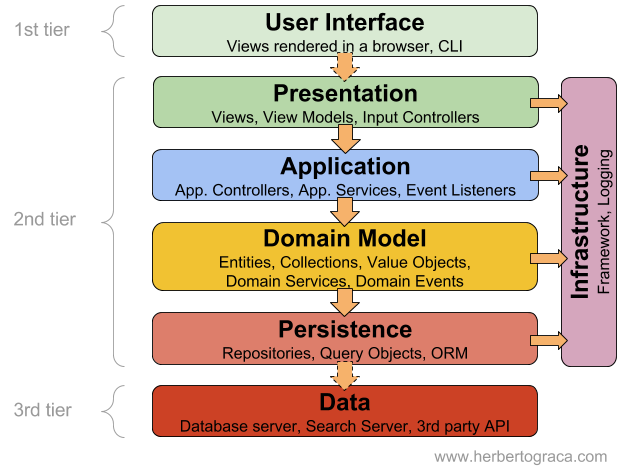
\includegraphics[width=1.0\linewidth]{fig03}
 \caption{Трислойна софтуерна архитектура}
\label{figure03}
\end{figure}
\FloatBarrier

Основната идея за разделяне на три слоя е възможността слоевете да бъдат подменяни в последствие. Примерно ако дълговременното съхранение на данните е реализирано на СУБД MySQL, но поради външни фактори се наложи миграция към СУБД PostgreSQL, то стриктното спазване на трислойната архитектура би направило подобна миграция бърза и с възможно най-малко дефекти. 

При трислойната архитектура обектният модел в средния слой съдържа работната логика на софтуера. Слоят за визуализация служи единствено за „моментна снимка“ на обектния модел и събирането на действията, които потребителят извършва в графичния потребителски интерфейс. Най-долният слой за дълготрайно съхранение на данните служи за опазване на информацията между отделни стартирания на изчислителната машина. Най-често в слоя за съхранение на данните се използва релационна система за управление на бази от данни, но все по-популярни стават и NoSQL системи. 

В контекста на трислойната архитектура има два основни подхода за разработката на софтуера, които се разделят по това кой от трите слоя ще бъде изработен първи. 

\begin{lstlisting}
https://herbertograca.com/2017/08/03/layered-architecture/
\end{lstlisting}

\subsection{Подход отгоре на долу (Top-Down)}

В някои ситуации е по-рационално първоначално да се създадат работните екрани от графичния потребителски интерфейс. Най-често това се случва, когато от хартиен документооборот се преминава към електронен документооборот и интегрирана информационна система. Причината за това е, че съществуват множество формуляри на хартия, които относително лесно могат да се пресъздадат в електронен вариант. Недостатък при този подхода на работа е, че когато се достигне до най-долния слой (дълговременното съхранение) е възможно един и същи данни да се появят дублирани на множество места (таблици в релационната база данни). 

\subsection{Подход отдоло на горе (Bottom-Up)}

Алтернативно решение е системата да бъде създадена от долния слой към горните. Тогава се прави обстоен анализ на информацията и се създава модел на данните. Първоначално се проектира модулът за дълготрайно съхранение (най-често релационна база данни), след което се създава обектен модел и едва след това графичният потребителски интерфейс. Недостатък при този подход е, че ако бъде пропусната съществена информация в най-долния слой, това значително затруднява последващи корекции на системата. 

\begin{lstlisting}
https://en.wikipedia.org/wiki/Top-down_and_bottom-up_design
\end{lstlisting}

\subsection{Избор на подход в настоящата разработка}

При настоящата разработка основно са налични няколко потребителски екрана, като основният екран е предназначен за визуализацията на игралното поле. В същото време относително малко количество информация се съхранява между отделни стартирания на софтуера. Поради тези два факта по-удачно е да се реализира подход „отгоре надолу“, което означава първоначално създаване на графичния потребителски интерфейс, след това изграждане на обектно ориентиран модел и едва накрая добавяне на релационна база данни. 

